\documentclass[]{llncs}

\usepackage{graphicx}
% Used for displaying a sample figure. If possible, figure files should
% be included in EPS format.
%
% If you use the hyperref package, please uncomment the following line
% to display URLs in blue roman font according to Springer's eBook style:
% \renewcommand\UrlFont{\color{blue}\rmfamily}

% Display polish characters
\usepackage[utf8]{inputenc}
\usepackage{polski}
\usepackage{url}
\pagestyle{plain}

\usepackage[language=polish, sorting=none]{biblatex}
\addbibresource{bibliography.bib}

% Translate some names to polish
\def\keywordname{{\bf Słowa Kluczowe:}}


\usepackage{letltxmacro}
\LetLtxMacro{\oldcite}{\cite}
% \renewcommand{\cite}[1]{\hspace{.25em}\oldcite{#1}}
\renewcommand{\cite}[1]{~\oldcite{#1}}

\LetLtxMacro{\oldfootnote}{\footnote}
\renewcommand{\footnote}[1]{~\oldfootnote{#1}}
\newcommand{\code}[1]{\texttt{#1}}

\begin{document}

\title{Wykorzystanie Ethereum do Budowy Zdecentralizowanej Aplikacji}
\author{Wojciech Korzeniowski}
\institute{
  Instytut Informatyki\\Wydział Elektroniki i Technik Informacyjnych\\Politechnika Warszawska\\
  \url{http://www.ii.pw.edu.pl/}
}

\maketitle

\makeatletter
\let\ps@oldempty\ps@empty % save default definition of \ps@empty
\renewcommand\ps@empty\ps@plain
\makeatother

\begin{abstract}

  Artykuł zaczyna się od opisu Ethereum jako platformy do definiowania smart
  kontraktów. W kolejnym rozdziale znajduje się opis możliwości smart kontraktów
  wraz z przykładem ich wykorzystania w postaci rozproszonego systemu do
  głosowania. Następnie opisany jest sposób komunikacji z siecią Ethereum z
  poziomu aplikacji przeglądarkowej. Ostatni rozdział traktuje o bezpieczeństwie
  i zagrożeniach wynikających z utraty kontroli nad danymi aplikacji.

  \keywords{Ethereum \and Smart kontrakt \and Blockchain \and Aplikacje
  Zdecentralizowane}

\end{abstract}

\section{Ethereum}

  Ethereum jest zdecentralizowaną platformą dla aplikacji, które działają
  dokładnie tak jak zostały zdefiniowane bez możliwości oszustwa, cenzury czy
  interwencji stron trzecich.\footnote{https://www.ethereum.org} Platforma została uruchomiona
  30~lipca~2015 przez rosyjskiego programistę nazywającego się Vitalik Buterin i
  jej główną funkcjonalnością jest możliwość definiowana smart kontraktów.

  Ether jest kryptowalutą wykorzystywaną na platformie Ethereum. Pod względem
  wartości rynkowej jest drugą co do wielkości kryptowalutą na świecie, zaraz po
  Bitcoinie.\footnote{Według serwisu \url{https://coinmarketcap.com/}, stan na
  2.06.2018} Bitcoin, uruchomiony 9 stycznia 2009 roku, został stworzony aby
  umożliwić transfer waluty bez ograniczeń w postaci instytucji bankowych czy
  lokalizacyjnych. Pomimo tego że również umożliwia definiowanie smart
  kontraktów, częściej do tego celu wykorzystywane jest Ethereum.

\section{Smart kontrakt}

  Smart kontrakt jest kolejnym etapem rozwoju zastosowań technologii blockchain.
  Można znaleźć tłumaczenia, które opisują smart kontrakt jako cyfrowy zapis
  umowy, która w odpowiednich warunkach realizuje ustaloną akcję. Z technicznego
  punktu widzenia jest to zbiór danych, które zostaną zachowane dopóki działa
  co najmniej jeden z węzłów sieci Ethereum, oraz funkcji, które mogą operować na
  danych i są jedynym sposobem na ich zmianę.

  Ta funkcjonalność spowodowała powstanie nowego rodzaju aplikacji oznaczanych
  DApp, od angielskiego terminu Decentralized Application, co oznacza w języku
  angielskim "zdecentralizowana aplikacja". Są to aplikacje, które wykorzystują
  smart kontrakty, lub bardziej ogólnie blockchain, jako miejsce do
  przechowywania kodu i danych aplikacji. W Ethereum smart kontrakty definiuje
  się wykorzystując język Solidity\cite{solidity-doc}.

  Wywołania niektórych funkcji wymagają przekazania Etheru, który może być
  przechowywany w smart kontrakcie jak w zwykłym portfelu lub być przekazanym
  dalej wraz z wywołaniem innej funkcji. Ma to miejsce na przykład w grach
  hazardowych gdzie aby wywołać funkcję losu należy przekazać ustaloną kwotę
  Etheru jako opłatę za los.

  Istotną cechą, która wynika z architektury blockchainu jest fakt, iż smart
  kontrakt, który został utworzony na blockchainie nie może zostać zmieniony.
  Jest to bardzo istotne ze względu na bezpieczeństwo tworzonej aplikacji.
  Jeżeli popełnimy błąd w definicji kontraktu nie ma możliwości jego naprawy.
  Jedyne co można zrobić to utworzyć nowy kontakt i zaprzestać korzystania z
  jego starej wersji. Takie rozwiązanie nie zawsze jest satysfakcjonujące,
  szczególnie jeżeli do starej wersji kontraktu przypisany jest Ether a nie
  utworzyliśmy funkcji, która pozwala na jego przekazanie do innego portfela. Z
  drugiej strony istnienie funkcji, która pozwala na wybranie całego Etheru z
  kontraktu może wzbudzić podejrzenia co do intencji jego twórcy.

  Funkcje zdefiniowane w smart kontrakcie można podzielić na dwie kategorie. Te,
  które czytają dane i te, które je zmieniają. Jako że dostęp do danych z
  blockchainu jest publiczny i można stworzyć własny węzeł, który jest pełną
  kopią blockchainu, dane można odczytać w każdej chwili. Inaczej jest w
  przypadku funkcji, która modyfikuje stan kontraktu lub samego tworzenia
  kontraktu. Wynika to z faktu, iż każdy z węzłów w sieci musi wywołać tę
  funkcję aby potwierdzić czy inne węzły również ją wykonały i stan blockchainu
  po wywołaniu funkcji się zgadza między węzłami. Fakt, iż musimy wykonać tę
  funkcję na wszystkich węzłach powoduje że za jej wywołanie, wołający musi
  zapłacić. Koszt operacji wyrażany jest w jednostce Gas. Ilość Gasu potrzebnego
  do wywołania funkcji jest proporcjonalna do złożoności obliczeniowej wołanej
  funkcji. Podczas tworzenia transakcji można określić ile maksymalnie Gasu może
  być wykorzystane na wywołanie funkcji. Jeżeli podczas wywoływania funkcji
  ustalony limit zostanie osiągnięty, wywołanie zostaje przerwane aby nie
  przekroczyć limitu.

  Wywołania funkcji, utworzenie smart kontraktu oraz transfer Etheru na inne
  konto nazywamy transakcją. Wszystkie transakcje trafiają do puli transakcji.
  Zazwyczaj kopacze podczas wykopywania nowego bloku wybierają z puli te
  transakcje, w których autor ustalił największą cenę za Gas. Dzieje się tak
  ponieważ to kopacz dostaję opłata za Gas ze wszystkich transakcji które
  wchodzą w skład nowo wykopanego bloku. Stąd cena Gasu zależy od aktualnego
  obciążenia sieci oraz od tego czy chcemy aby nasza funkcja została wywołana
  jak najszybciej. Po ustaleniu zbyt niskiej ceny za transakcję może się zdążyć
  tak, że kopacze będą wybierać bardziej korzystne dla nich transakcje powodując
  że transakcja może znajdować się w puli transakcji przez bardzo długi
  czas.\footnote{\url{https://ethgasstation.info/} – serwis estymujący opłatę za
  transakcję }

  \subsection{System do głosowania}

  Smart kontrakty mogą zostać wykorzystane do zbudowania systemu do tajnego
  głosowania. Organizator głosowania tworzy umowę z osobami uprawnionymi do
  głosowania, która pozwala uprawnionym na oddanie dokładnie jednego głosu.
  Następnie, po zamknięciu głosowania, opcja, która zebrała najwięcej głosów
  zostaje zwycięzcą głosowania.

  Zastanówmy się najpierw jakie są problemy w organizowaniu głosowania bez smart
  kontraktów. Przede wszystkim należy zadbać o to aby głos mogła oddać tylko
  osoba do tego upoważniona oraz aby każda z tych osób mogła oddać tylko jeden
  głos. Kolejnym problemem jest sposób w jaki głosy są liczone. Jak powiedział
  Józef Stalin: "Nieważne, kto głosuje, ważne, kto liczy głosy."

  Powyższe problemy w przypadku głosowań w Polsce rozwiązywane są przez
  Państwową Komisję Wyborczą, która organizuje i pilnuje porządku głosowania.
  Tworzone są okręgowe komisje wyborcze, których odpowiedzialnością jest
  kontrolowanie czy osoba oddająca głos jest do tego uprawiona. Następnie
  komisja skrutacyjna liczy głosy po czym ogłaszany jest wynik głosowania.

  Takie rozwiązanie wymaga istnienia tak zwanej "zaufanej trzeciej strony". W
  przypadku wyborów w Polsce jest to PKW. Obywatele muszą zaufać że komisja w
  poprawny sposób zorganizuje i przeprowadzi głosowanie a następnie bezbłędnie
  policzy głosy i ogłosi zwycięzcę.  Nie raz pojawiały się różnego rodzaju
  kontrowersje co do sposobu przeprowadzania wyborów. Na przykład podczas
  wyborów samorządowych 2014 opóźnione było ogłoszenie wyników.  PKW tłumaczyła
  to awarią systemów informacyjnych jednak co bardziej podejrzliwi obywatele
  wyczuwali w tym spisek. Dodatkowo obywatele muszą ufać że każda z okręgowych
  komisji wyborczych będzie przestrzegać prawa i nie nadużyje swoich kompetencji
  aby sfałszować organizowane wybory.

  W przypadku głosowania zrealizowanego na smart kontraktach nie ma potrzeby
  istnienia zaufanej trzeciej strony. Można zdefiniować kontrakt, którego
  definicja jest publicznie dostępna i każdy może sprawdzić w jaki sposób
  zbierane są głosy oraz jak są one zliczane. Wymaganie aby każdy z uprawionych
  mógł zagłosować tylko jeden raz można zrealizować poprzez przekazanie każdemu
  uprawnionemu jednego tokenu do głosowania, który nie może być przekazany
  dalej.  Osoba, która wykorzystuje swój token do zagłosowania wywołuje
  odpowiednią funkcję na kontrakcie do głosowania w efekcie czego liczba głosów
  na wybraną opcję zwiększa się.

  Jedną z głównych zalet realizacji systemu głosowania opartego na blockchainie
  jest jego transparentność. Ponieważ dane zapisane na blockchainie są
  publicznie dostępne do odczytu każdy z zainteresowany może sprawdzić jak
  przebiegało głosowanie oraz jaki jest jego aktualny stan. Ponadto technologia
  blockchain gwarantuje że dane zapisane w blockchainie nie zostaną zmienione
  więc nie ma możliwości fałszowania wyników.

\section{Token}

  Tokenem w świecie Ethereum nazywamy nową "kryptowalutę", która istnieje na
  blockchainie Ethereum. Istnieje przyjęty interfejs tokenu o nazwie `ERC20`,
  którego implementacja musi definiować między innymi całkowitą liczbę tokenów,
  nazwę oraz zasady przekazywania go innym użytkownikom.

  Tokeny mogą być wykorzystane do zbiórki pieniędzy co jest nazywane ICO (ang.
  Initial Coin Offering) i jest odpowiednikiem określenia IOP (ang. Initial
  Public Offering) znanego giełd papierów wartościowych. Przypuśćmy że
  właściciel startupu potrzebuje dofinansowania do swojego biznesu. Może on
  utworzyć token, który następnie będzie sprzedawał za Ether. W ten sposób
  twórca pozyskuje Ether, którym może płacić lub wymienić na inną walutę.
  Natomiast kupujący w zależności od przyjętej polityki ICO, może otrzymać
  udziały w startupie lub możliwość wykorzystania tokenu w zamian za usługę
  realizowaną przez biznes twórcy tokenu. Podczas ICO cena tokenu jest ustalana
  przez jego twórce, w późniejszym czasie jego wartość jest weryfikowana przez
  rynek.

\section{Komunikacja z siecią Ethereum}

  Sieć Ethereum\cite{ethereum-doc} składa się z węzłów. Węzeł to serwer, który
  posiada lokalną kopię blockchainu wraz ze wszystkimi transakcjami i smart
  kontraktami, które zostały w nim zapisane. Węzły komunikują się ze sobą w celu
  ustalenia jednej, wspólnej wersji blockchainu, jest to nazywane ustaleniem
  konsensusu. Najbardziej rozpowszechnionym sposobem ustalenia konsensusu, który
  jest wykorzystywany zarówno w Ethereum jak i w Bitcoinie, jest dowód pracy. W
  związku z ogromnym zużyciem energii elektrycznej które jest wymagane przed
  dowód pracy jedną z propozycji rozwoju Ethereum jest zmiana sposobu ustalania
  konsensusu i przejście na dowód stawki.\cite{proof-of-stake}

  Aby utworzyć własny węzeł Ethereum można wykorzystać oficjalną implementację
  węzła, dostępną do pobrania z serwisu
  Github\footnote{\url{https://github.com/ethereum/go-ethereum}}. Nie jest to jednak
  koniecznie jeżeli chcemy zacząć przygodę z tworzeniem smart kontraktów. Serwis
  Infura\footnote{\url{https://infura.io/}} udostępnia za darmo publiczny węzeł, który
  można wykorzystać do komunikacji z siecią Ethereum. Komunikacja z węzłem
  następuje przy pomocy protokołu JSON-RPC. Jednym z bardziej znanych klientów
  jest klient napisany w języku JavaScript o nazwie
  Web3.js\footnote{\url{https://github.com/ethereum/web3.js/}}. Wykorzystując go można
  stworzyć aplikację działającą w przeglądarce, która komunikuje się
  bezpośrednio z węzłem Ethereum.

  Aby utworzyć własny kontrakt w sieci można skorzystać z narzędzia
  Remix\footnote{\url{https://remix.ethereum.org/}}. Jest to edytor w, którym można
  napisać własny kontrakt a następnie z poziomu przeglądarki utworzyć jego kopię
  na blockchainie. Aby możliwe było utworzenie kontraktu na blockchainie twórca
  musi musi ponieść koszt utworzenia kontraktu. W przypadku narzędzia Remix oraz
  innych aplikacji przeglądarkowych wykorzystujących klienta Web3.js można
  skorzystać z wtyczki do przeglądarki o nazwie
  Metamask\footnote{\url{https://metamask.io/}}.

  Technicznie Metamask wstrzykuje do strony globalny obiekt JavaScript o nazwie
  \code{web3}, który jest wykorzystywany do dalszej interakcji z blockchainem. Podczas
  tworzenia nowego smart kontraktu lub wywoływania funkcji, która wymaga zapłaty
  pojawia się okienko, które wymaga potwierdzenia czy chcemy wykonać daną akcję
  za określoną opłatą.

\section{Architektura aplikacji}

  Najprostszą architekturą DApp jest klient działający w przeglądarce, który
  komunikuje się bezpośrednio z wybranym węzłem. Inną możliwością jest
  stworzenie własnego serwera, który komunikuje się z węzłem oraz aplikację
  przeglądarkową komunikującą się tylko z naszym serwerem bez bezpośredniej
  komunikacji z węzłem. Takie rozwiązanie może być wykorzystane w celu
  przyspieszenia aplikacji aby nie odpytywać węzeł o dane za każdym razem tylko
  przechowywać je w pamięci podręcznej na serwerze.

  Innym sposobem na wykorzystanie blockchainu jest wykorzystanie go tylko do
  przechowywania wartości funkcji skrótu danych, które trzymamy w innym miejscu.
  Takie podejście stosowane jest ze względu na fakt, że zapis do blockchainu
  kosztuje proporcjonalnie do złożoności obliczeniowej wywoływanej funkcji a w
  przypadku zapisu wartości funkcji skrótu koszt jest stały oraz nie zależy od
  ilości danych, z których powstał skrót. Blockchain w takim przypadku służy
  tylko do weryfikacji czy dane, które odczytujemy zgadzają się z danymi, które
  zostały "podpisane" poprzez zapisanie ich skrótu na blockchainie.

\section{Bezpieczeństwo}

  Dane aplikacji są najczęściej centralnym punktem stworzonej aplikacji, co
  powoduje że stają się celem ataków grup hakerskich. Utrata danych może
  spowodować że aplikacja staje się mniej wygodna w
  użytkowaniu\cite{teatr-wspolczesny-utrata-danych} a także sprawić że
  użytkownicy tracą zaufanie do twórców aplikacji\cite{nazwa-pl-utrata-danych}.
  Dane mogą także wyciec\cite{wyciek-danych-studentow}, w takim
  przypadku aplikacja działa jak przed atakiem jednak dane aplikacji zostały
  upublicznione lub przekazane osobom które nie powinny mieć do nich dostępu.

  Ciężko ocenić, który ze scenariuszy jest gorszy. Usunięcie danych może
  sparaliżować pracę użytkownika aplikacji lub nawet nieść konsekwencje prawne w
  przypadku utraty wrażliwych danych, które są nie do odzyskania np.
  dokumentacji podatkowych\cite{utrata-dokumentacji}. W przypadku utraty danych
  możemy przewidzieć jakie konsekwencje się z tym wiążą. Inaczej jest gdy
  nastąpi wyciek danych. Zdarzają się sytuacje, w których serwis świadomie lub
  nie, udostępnia czyjeś dane. W takim przypadku ciężko jest przewidzieć w jaki
  sposób dane użytkowników mogą zostaną użyte. Z problemem wycieku danych
  musiało zmierzyć się Poznańskie Centrum Superkomputerowo-Sieciowe, które
  pozwalało na pobranie imienia, nazwiska oraz adresu zamieszkana po podaniu
  numeru PESEL\cite{dane-dzieci}.

  Wykorzystanie technologii blockchain pozwala ograniczyć wymienione powyżej
  zagrożenia ponieważ usunięcie danych z blockchainu jest niemożliwe. Ciężko
  też mówić o wycieku danych ponieważ dane zapisane na blockchainie są
  publicznie dostępne. Oczywiście jeżeli chcemy przechowywać dane wrażliwe na
  blockchainie muszą one być zaszyfrowane i możliwe do odczytu tylko dla
  odpowiednich osób. Jeżeli szyfrowanie zostanie zrealizowane błędnie lub sam
  klucz szyfrujący zostanie przejęty przez atakującego możemy mówić o wycieku
  danych.

  Dodatkowo jak wspomniałem w rozdziale 5, DApp może wykorzystywać tradycyjne
  bazy danych takie jak relacyjne czy NoSQL. W takim przypadku twórcy aplikacji
  muszą brać pod uwagę zarówno niebezpieczeństwa związane z wykorzystaniem
  wybranej bazy danych jak i te wynikające z użycia blockchainu.

  W celu wykorzystania sprawdzonych rozwiązań na problemy, które często się
  powtarzają podczas projektowania smart kontraktów warto skorzystać ze zbioru
  OpenZeppelin\footnote{\url{https://github.com/OpenZeppelin/zeppelin-solidity}}.
  Można znaleźć tam gotowe smart kontrakty lub funkcje, które rozwiązują dane
  problemy bezpieczeństwa w sprawdzony przez społeczność Ethereum sposób.
  Przykładem może być chęć ograniczenia możliwości wywołania niektórych funkcji
  tylko do autora danego smart kontraktu. Jedną z takich funkcji może być
  wspomniana wcześniej funkcja służąca do wybrania Etheru, który jest
  przechowywany na smart kontrakcie.

  % \subsection{Generowanie liczb pseudolosowych}\cite{liczby-losowe}

% \cite{liczby-losowe}

\section{Podsumowanie}

  Blockchain oraz smart kontrakty mogą usprawnić funkcjonowanie instytucji które
  zajmują się przetwarzaniem pieniędzy. Działania które do tej pory należało
  wykonać ręcznie lub wymagały zaufania od użytkowników przy pomocy odpowiednio
  zdefiniowanego kontraktu mogą być wykonywane automatycznie. Giełdy
  kryptowalutowe są jedną z pierwszych instytucji które praktycznie w pełni
  działają w oparciu o smart kontrakty. Dzięki temu mamy pewność że giełda
  działa za każdym razem tak samo i nie popełni błędu, który może wynikać ze
  zwykłej pomyłki jak i celowego oszustwa.

  Wykorzystanie smart kontraktów pozwala na wyeliminowanie wymagania istnienia
  zaufanej trzeciej strony, jeżeli serwis udostępnia kod źródłowy kontraktu
  możemy go przeczytać, zrozumieć i mieć pewność że nigdy nie zostaniemy
  oszukani przy jego pomocy. Dzięki spisaniu zasad umowy w postaci kodu
  źródłowego mamy gwarancję, że umowę można zinterpretować tylko w jeden sposób
  oraz pewność wykonania danych akcji po spełnieniu wcześniej przyjętych
  warunków.

\printbibliography
\end{document}

% ########## START OF SAMPLES

% \newpage
% \newpage

% \section{Takie tam przydatne przykłady}
% \begin{definition} text \end{definition}
% \begin{case} text \end{case}
% \begin{proof} text \end{proof}

% \noindent Widać na równaniu:
% \begin{equation}
%   x + y = z
% \end{equation}

% Please try to avoid rasterized images for line-art diagrams and
% schemas. Whenever possible, use vector graphics instead (see
% Fig.~\ref{fig1}).

% \begin{figure}
%   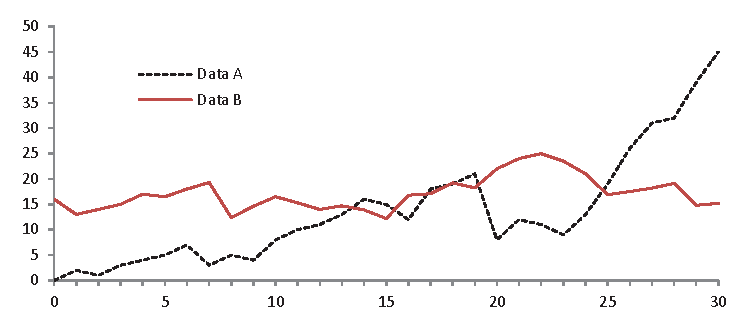
\includegraphics[width=\textwidth]{fig1.eps}
%   \caption{A figure caption is always placed below the illustration.
%     Please note that short captions are centered, while long ones are
%   justified by the macro package automatically.} \label{fig1}
% \end{figure}

% Tabla~\ref{tab1} przedstawia że działa.

% \begin{table}
%   \caption{Table captions should be placed above the
%   tables.}\label{tab1}
%   \begin{tabular}{|l|l|l|}
%     \hline
%     Heading level &  Example & Font size and style\\
%     \hline
%     Title (centered) &  {\Large\bfseries Lecture Notes} & 14 point, bold\\
%     1st-level heading &  {\large\bfseries 1 Introduction} & 12 point, bold\\
%     2nd-level heading & {\bfseries 2.1 Printing Area} & 10 point, bold\\
%     3rd-level heading & {\bfseries Run-in Heading in Bold.} Text follows & 10 point, bold\\
%     4th-level heading & {\itshape Lowest Level Heading.} Text follows & 10 point, italic\\
%     \hline
%   \end{tabular}
% \end{table}

% % ########## END OF SAMPLES
